\documentclass
[handout]
{beamer}

%%
%%
%%
% From http://tex.stackexchange.com/questions/2072/beamer-navigation-circles-without-subsections
% Solution #2 or 3:
% \usepackage{etoolbox}
% \makeatletter
% % replace the subsection number test with a test that always returns true
% \patchcmd{\slideentry}{\ifnum#2>0}{\ifnum2>0}{}{\@error{unable to patch}}%
% \makeatother
% Solution #1:
\usepackage{remreset}% tiny package containing just the \@removefromreset command
\makeatletter
\@removefromreset{subsection}{section}
\makeatother
\setcounter{subsection}{1}


\usepackage{etex}
\usepackage{pgf}
\usepackage{tikz}
\usepackage{url}
\usepackage{amsmath}
\usepackage{color}
% \definecolor{red}{rgb}{1,0,0}
\usepackage{ulem}
% \usepackage{booktabs}
\usepackage{colortbl,booktabs}
\renewcommand*{\thefootnote}{\fnsymbol{footnote}}
\usepackage{fancybox}
\usepackage[framemethod=TikZ]{mdframed}
\mdfdefinestyle{FactStyle}{%
  outerlinewidth=0.5,
  roundcorner=1pt,
  leftmargin=1cm,
  linecolor=blue,
  outerlinecolor=blue!70!black,
  backgroundcolor=yellow!40
}
\usepackage{cancel}

  \newcommand\Warning{%
    \makebox[2.4em][c]{%
      \makebox[0pt][c]{\raisebox{.2em}{\Large!}}%
      \makebox[0pt][c]{\color{red}\Huge$\bigtriangleup$}}}%

\usepackage{stackengine}
\usepackage{scalerel}
\usepackage{xcolor}
  \newcommand\dangersign[1][2ex]{%
    \renewcommand\stacktype{L}%
    \scaleto{\stackon[1.3pt]{\color{red}$\triangle$}{\tiny !}}{#1}%
  }



\usepackage{dcolumn}
\newcolumntype{d}[1]{D{.}{.}{#1}}

% From
% http://tex.stackexchange.com/questions/109900/how-can-i-box-multiple-aligned-equations
\usepackage{empheq}
\usepackage{tcolorbox}  \newtcbox{\othermathbox}[1][]{%
  nobeforeafter, tcbox raise base, 
  colback=black!10, colframe=red!30, 
  left=1em, top=0.5em, right=1em, bottom=0.5em}

\newcommand\blue{\color{blue}}
\newcommand\red{\color{red}}
\newcommand\green{\color{green!75!black}}
\newcommand\purple{\color{purple}}
\newcommand\bluegreen{\color{blue!75!green}}
\newcommand\orange{\color{orange}}
\newcommand\redgreen{\color{red!50!green}}
\newcommand\grey{\color{black}}
\newcommand\gap{\vspace{.1in}}
\newcommand\nb{${\red\bullet}\ $}
\newcommand\halfgap{\vspace{.05in}}
\newcommand\divideline{\line(1,0){352}}
\usepackage{marvosym} % for \Smiley

\newcommand{\bluealert}[1]{{\blue\textbf{#1}}}

% \usepackage{beamerthemesplit} %Key package for beamer
\usetheme{Singapore}
% \usetheme{Szeged}
% \usetheme{Garfield}
% \usetheme{CambridgeUS}
% \usenavigationsymbolstemplate{} %Gets rid of slide navigation symbols


\setbeamercolor{separation line}{use=structure,bg=structure.fg!50!bg}
% \begin{beamercolorbox}[colsep=0.5pt]
%   {upper separation line foot}
% \end{beamercolorbox}



\makeatletter
\setbeamertemplate{footline}
{
  \leavevmode%
  \hbox{%
% \begin{beamercolorbox}[colsep=0.5pt]
%   {upper separation line foot}
% \end{beamercolorbox}


  \begin{beamercolorbox}[wd=.5\paperwidth,ht=2.25ex,dp=2ex,colsep=0.5pt]%
    {upper separation line foot}
    \usebeamerfont{author in head/foot}%
    \hspace*{2ex}\insertshortdate:\ \insertshorttitle
  \end{beamercolorbox}%
  \begin{beamercolorbox}[wd=.5\paperwidth,ht=2.25ex,dp=2ex,right]{title in head/foot}%
    \usebeamerfont{title in head/foot}
    {\insertshortauthor}\hspace*{2ex}
  \end{beamercolorbox}}%
  % \begin{beamercolorbox}[wd=.333333\paperwidth,ht=2.25ex,dp=2ex,right]{date in head/foot}%
  %   \usebeamerfont{date in head/foot}\insertshortdate{}\hspace*{2em}
  %   \insertframenumber{} / \inserttotalframenumber\hspace*{2ex} 
  % \end{beamercolorbox}%
  \vskip0pt%
}
\makeatother

\usetikzlibrary{decorations.markings}
\usetikzlibrary{arrows}


\title{Final Exam Review}
\author{Peter Garfield, UCSB Mathematics}
\date{March 15, 2017}
%\institute{}


\useinnertheme{default}

\usefonttheme{serif}
% \usecolortheme{rose}
% \usecolortheme{whale}
% \usecolortheme{orchid}
\usecolortheme{crane}
% \usecolortheme{dolphin}


%TEMPLATE
\setbeamertemplate{navigation symbols}{}

\setbeamertemplate{note page}[compress]

\setbeamertemplate{frametitle}{
  \vspace{0.5em}
  % \begin{centering}
  {\huge\blue\textbf{\textmd{\insertframetitle}}}
  \par
  % \end{centering}
}

% From http://tex.stackexchange.com/questions/7032/good-way-to-make-textcircled-numbers:
\newcommand*\circled[1]{\tikz[baseline=(char.base)]{\node[shape=circle,draw,fill=orange,inner sep=1pt] (char) {#1};}} 
% \renewcommand{\labelenumi}{\circled{\textbf{\arabic{enumi}}}}

\let\olddescription\description
\let\oldenddescription\enddescription
\usepackage{enumitem}
\let\description\olddescription
\let\enddescription\oldenddescription

% \usepackage[loadonly]{enumitem}
\setlist[enumerate,1]{label=\colorbox{orange}{\arabic*.},font=\bfseries}
%\setlist[enumerate,2]{label=\colorbox{blue!25}{(\alph*)},font=\bfseries}
% \setlist[enumerate,1]{label=\arabic*.,font=\bfseries}
\setlist[itemize,1]{label=\red$\bullet$}
\setlist[itemize,2]{label=\blue$\bullet$}

\newcommand\answer[1]{\fbox{#1}}
% \renewcommand\answer[1]{}

\newcommand{\antilog}{\operatorname{antilog}}








\title{}
\title{Logarithm Applications}
\date{April 26, 2022}


\begin{document}
\small



\section*{Administration}

\frame{
  \frametitle{}
  {\Huge{}Welcome Back!}\\[.5em]

  {\Huge{}Differential Calculus}
  \vfill
  {\Large{}Instructor:}\\
  \ \hspace*{0.2in} Nathan Schley ({\it Sh}+{\it lye}), \url{schley@math.ucsb.edu}\\
  \ \hspace*{0.2in} South Hall 6701
  \\[0.5em]

  {\Large{}Office Hours:}\\
  \ \hspace*{0.2in} T R 11-11:50, T 3:45-4:35 Details on Gauchospace. 
  \bigskip

  \copyright\ 2022\ Daryl Cooper, Peter M.\ Garfield, Ebrahim Ebrahim \& Nathan Schley\\
  Please do not distribute outside of this course.
  \vfill

}

\frame{
  \frametitle{Counting and Our Logarithmic Perception of the World}
Vsauce: 1,2,3,4,5,6,7,8,9,10,11,12,13,14,15,16,17,18,19,20,21,22,23,24,25,26,27,\\
28,29,30,31,32,33,34,35... \\
https://www.youtube.com/watch?v=Pxb5lSPLy9c


}

\frame{
  \frametitle{Warm-up}

  \begin{itemize} 
  \item $\log_9(9^4) = $ \pause \ \ \fbox{4}
  \pause
  \item $\log_3(9^4) = $ \pause \ \ \fbox{8}
  \pause
  \item $\log_{27}(27^5) = $ \pause \ \ \fbox{5}
  \pause
  \item $\log_3(27^5) = $ \pause \ \ \fbox{15}
  \pause
  \item $\log_5(25^{17}) = $ \pause \ \ \fbox{34}
  \pause
  \item $\log_3(27^0) = $ \pause \ \ \fbox{0}
  \pause
  \item $\log_8(2^{12}) = $ \pause \  \fbox{4}
  \item $\log_8(2) = $ \pause \  \fbox{1/3}
  
  \end{itemize}
  
  
  

} 

\frame{
  \frametitle{Warm-up Part II}

  \pause   
  \begin{itemize} 
  \item $\log_{100}(100^7) = $ \pause \ \ \fbox{7}
  \pause
  \item $\log_{10}(100^7) = $ \pause \ \ \fbox{14}
  \pause
  \item $\log_{10}(1000000^{-4}) = $ \pause \ \ \fbox{-24}
  \pause
  \item $\log_{10}(2) = $ \pause \  about \ \fbox{.3}
  \pause \ \ \ \ {\red Still warm-up?} \pause
  \item $\log_{10}(2^{11}) =  \pause \ \ $ about $ .3\cdot 11 $ \pause $=$ \fbox{3.3} \pause \\ 
  
  \end{itemize}
  
  
}  


\section*{Log Rules}



\frame{

logs are ``{\blue opposite} '' of exponents (inverse function of antilog)\\
So every fact about exponents corresponds to a fact about logs:

\gap

\begin{table}
\begin{tabular}{lll}
 & {\blue laws of exponents} & {\blue corresponding law of logs} \\\toprule
{\red(1)}  & $10^{\red a}\times10^{\red b} = 10^{{\red a}+{\red b}} $ & 
$\log({\blue x y})= \log({\blue x})+\log({\blue y})$ \\
{\red(2)} & $10^{\red 0} = {\blue 1}$ & $\log({\blue 1}) ={\red 0}$\\
{\red(3)} & $10^{\red -a} = 1/10^{\red a}$ & $\log({\blue 1/x}) =-\log({\blue x})$\\
{\red(4)} & $\left(10^{\red a}\right)^{\red p} = 10^{\red ap}$ & $\log({\blue x}^{\red p}) ={\red p}\log({\blue x})$\\
{\red(5)}  & $10^{\red a}/10^{\red b} = 10^{{\red a}-{\red b}} $ & $\log({\blue x/y})= \log({\blue x})-\log({\blue y})$ 
\end{tabular}
\end{table}

Example: $\log(x^a/y^b)=$?
\begin{center}
  $A = a\log(x)/(b\log(y))\qquad B = a\log(x) + b\log(y)$\\
  $C = a\log(x)-b\log(y)\quad D =(a+\log(x))-(b+\log(y))$
  \pause
  \fbox{C}   
\end{center}

}

\frame{
  \frametitle{Rule (4): $\log(x^p) = p \log(x)$}

  Explanation of {\purple (4)}
  \gap

  $\log(a\times a)=\log(a)+\log(a) = {\red 2}\log(a)$\\ \pause
  $\log(a\times a\times a)=\log(a)+\log(a) + \log(a)={\red 3}\log(a)$ \\ \pause
  \gap
  
  In general:  the number of tens you multiply to get $x^{\red p}$ is ${\red p}$ times as many tens as you multiply to get $x.$
  \gap

  What is $\log\left(\sqrt{\frac{1}{x^7}}\right)$?
  \begin{center}
    $A = 7-\log(x)\quad B = (7/2)-\log(x)\quad C = -7/2\quad D = -(7/2)\log(x)$\quad\pause\fbox{D}
  \end{center}


}

\frame{


Find $x$ by solving $3^{x} = 5$.\\[2em]
    
      A\ \ $\log(5)/\log(3)$
      \\
      B\ \ $\log(3)/\log(5)$
      \\
      C\ \ $\log(5)^3$
      \\
      D\ \ $\log(3)-\log(5)$
      \\
      E\ \ $\log(5)-\log(3)$
      \pause
      \qquad
      \fbox{A}
    




}



\section*{Log Arithmetic}

\frame{
  \frametitle{\S7.5: Using logs to multiply}

  First rule of logs:\  $\log(a{\blue \times }b)= \log(a){\blue +}\log(b)$
  \gap

  Example: Find $2.7\times 1.6$ using logs

  {\red{}Given info:}\ $\log(2.7)\approx 0.43$ and $\log(1.6)\approx 0.20$
  \gap


  {\blue Method}\\
  {\red(i)}\ Look up $\log(2.7)$ and $\log(1.6)$\\
  {\red(ii)}\ Add these\\
  {\red(iii)}\ Take the ${\red\mbox{antilog}}$ of result from (ii)\\
  {\red(iv)}\ Think: Is the answer {\red reasonable} or did I goof up?\\


  \vspace*{4in}

}


\frame{
  \frametitle{\S7.5: Using logs to multiply}

  First rule of logs:\  $\log(a{\blue \times }b)= \log(a){\blue +}\log(b)$
  \gap

  Example: Find $2.7\times 1.6$ using logs

  {\red{}Given info:}\ $\log(2.7)\approx 0.43$ and $\log(1.6)\approx 0.20$
  \gap

  {\blue Look how I write the answer.}
  \smallskip

  \begin{itemize}
  \item $\log(2.7{\red \times}1.6) {\blue =} \log(2.7){\red
      +}\log(1.6)$
    \pause

  \item We are told $\log(2.7){\blue \approx} 0.43$ and $\log(1.6){\blue \approx} 0.20$,
    so $\log(2.7{\red \times}1.6){\blue \approx} 0.43{\red +}0.20 =
    {\green 0.63}$
    \pause

  \item {\purple Is this the answer ?}\pause\  {\large{ \red Heck
        No!}} It is the {\red log} of the answer\\ 
    \pause

  \item $2.7{\red \times}1.6 \approx {\red\mbox{antilog}}({\green 0.63})=10^{\green 0.63}$

  \item  $10^{\green 0.63} \approx 4.3$\\

  \item Is my answer \fbox{4.3} reasonable? Yes, about $2\times 2=4$.
  \end{itemize}
  \vspace*{1in}

}









\frame{
  \frametitle{\S7.5: Using logs to divide}

  Remember Log Rule (5): \fbox{$\log(a{\blue\div} b) = \log(a){\blue -}\log(b)$}
  \gap

  \alert{Example:}\ Use this rule to find $38.2/1.77$

  {\red{}Given info:}\ $\log(3.82)\approx 0.58$ and $\log(1.77)\approx 0.25$
  \gap
  
  {\blue Method}\\
  {\red(i)}\ Look up $\log(3.82)$ and $\log(1.77)$, find $\log(38.2)$\\
  {\green $\star$You can find $\log(38.2)$ by adding 1 to $\log(3.82)$ because \\ 38.2 is 3.82 times \emph{one more} power of 10.$\star$} \\ 
  {\red(ii)}\ {\red{}Subtract!}\\
  {\red(iii)}\ Take the ${\red\mbox{antilog}}$ of result from (ii)\\
  {\red(iv)}\ Think: Is the answer {\red reasonable} or did I goof up?\\
  \begin{center}
    A$= \text{done}$
    \qquad
    B$=\text{confused}$
  \end{center}
  \vspace*{2in}

}








\frame{
  \frametitle{Powers Using Logs}

  Or, exploting Log Rule (4):
  \begin{empheq}[box=\othermathbox]{align*}
    \log(a^{\red p}) = {\red p}\log(a)
  \end{empheq}
  \gap
  Use this and the graph of $y=10^x$ to find $\sqrt{70}$.

  {\large\blue{}One Approach:}
  \begin{itemize}
  \item[\red(i)] Use graph and move decimal point trick to find
    $\log(70)$ \\ 
  {\green $\star$I will show the graph of the exponential function $10^x$ and talk about this method on Thursday.$\star$}
  \item[\red(ii)] $\log(\sqrt{70})=\log(70^{\red 1/2}) =({\red 1/2})\log(70)$


  \item[\red(iii)] Take the {\red$\antilog$}\ of result from
    {\red(ii)}

  \item[\red(iv)] Think: Is the answer {\red reasonable} or did I goof up?

  \end{itemize}
  \textbf{Hint:}\ $\log(7)\approx 0.84$

  \begin{center}
    A$=\text{done}$
    \quad
    B$=\text{working}$
    \quad
    C$=\text{confused}$
  \end{center}
  \pause

  Answer: $\sqrt{70} \approx 8.3$.  Is that reasonable?
  \vspace*{2in}

}

\frame{
  \frametitle{Computer Applications}

  One kilobyte ($1$\ {\red{}KB})\ is $2^{10}$.  
  \halfgap

  \alert{Problem:}\ Calculate $2^{10}$ using logs.
  \qquad 
  \textbf{Hint:}\ $\log(2)\approx 0.3$

  \begin{center}
    A$\approx 3$
    \quad 
    B$\approx 10.3$
    \quad 
    C$\approx 30$
    \quad 
    D$ \approx 1000$
    \quad 
    E$\approx 1100$
    \pause
    \qquad 
    \fbox{D}    
  \end{center}

  So: $2^{10} \approx 10^3 = 1000$ (really $2^{10} = 1024$).
  \vspace*{-1em}

  \begin{align*}
    \text{{\red 1KB} is really}\ 2^{10}
    & =1024 \approx 10^{\red 3}
    && \text{({\red K} is {\red K}ilo = thousand)}\\
    \text{{\red 1MB}  is really}\ 2^{20}
    & = \left(2^{10}\right)^2\approx(10^3)^2=10^{\red 6}
    && \text{({\red M} is {\red M}ega = million)}\\
    \text{{\red 1GB} is really}\ 2^{30}
    & =\left(2^{10}\right)^3\approx(10^3)^3=10^{\red 9}
    && \text{({\red G} is {\red G}iga = billion)}\\
    \text{{\red 1TB} is really}\ 2^{40}
    & =\left(2^{10}\right)^4\approx(10^3)^4=10^{\red 12}
    && \text{({\red T} is {\red T}era = trillion)}
  \end{align*}
  \vspace*{-1em}
  \pause

  Example: suppose on a certain island the population of rabbits
  doubles every generation.  After $20$ generations it
  multiplies by\ldots\pause\ $2^{20}\approx $ 1 million.
  \pause
  \gap 
  
  Powers of $2$ are easy to do, even in your head. To work out
  $2^{\red n}$ the {\blue log} of the answer is approximately
  $0.3{\red n},$ so $2^{\red n}$ is $1$ followed by $0.3{\red n}$
  zeroes.


}


% \section*{Interlude}

% \frame{
%   \frametitle{Interlude...}

% What can we learn from the \emph{graph} of $\log(x)$?
% }

\section*{Solving Equations}

\frame{
  \frametitle{\S7.7: Solving Exponential Eq'ns}

  \begin{enumerate}
  \item   Find $x$ by solving $10^{x} = 5$.
    \begin{center}
      A$=5$
      \quad 
      B$=0.5$
      \quad
      C$=\log(5)$
      \quad
      D$=\log(0.5)$
      \quad
      E$=\log(5)-\log(10)$
      \pause
      \qquad
      \fbox{C}
    \end{center}
  \end{enumerate}
  \pause

  {\Large\blue{}Look how I write the answer!}
  \begin{align*}
    \log(10^{x})
    & =\log(5)
    & & \text{\blue Take logs of both sides}\\
    x = \log(10^{x})
    & =\log(5)
    & & \text{\blue Using $\log(a^{\red p})={\red p}\log(a)$ and $\log(10)=1$}
  \end{align*}
  \pause
  % \gap





}

\frame{
  \frametitle{Examples:}

  Use the Fourth Law:
  \begin{empheq}[box=\othermathbox]{align*}
    \log(a^{\red{}x})={\red{}x} \log(a)
  \end{empheq}
  Slogan: Logs bring exponents down to ground level. 
  \gap 

  % If ${\red x}$ is the unknown you can't find it until it is at {\blue ground level}\\
  % So with these equations the first step is always to write on the paper \\ {\blue Take logs of both sides}.
  % \gap  

  \begin{enumerate}
    \setcounter{enumi}{1}
  \item Solve $3^{\red x} = 7$
    \begin{center}
      A$=\log(7/3)$
      \quad 
      B$ = \log(7)-\log(3)$
      \quad 
      C$=\log(7)+\log(3)$
      \\
      D$ =\log(3)/\log(7)$
      \quad 
      E$=\log(7)/\log(3)$
      \pause
      \quad 
      \fbox{E}
    \end{center}
  \end{enumerate}
  \gap

  {\large\blue Look how I write the answer:}
  \begin{align*}
    \log(3^{x})
    & =\log(7)
    && \text{\blue Take logs of both sides}\\
    x\log(3)
    =\log(3^{x})
    & = \log(7)
    && \text{\blue Using $\log(a^{\red{}p})={\red{}p}\log(a)$} \\
    \text{So:}\qquad 
    x & = \log(7)/\log(3)
  \end{align*}
  \vspace*{1in}

}

\frame{
  \frametitle{Examples:}

  Use the Fourth Law:
  \begin{empheq}[box=\othermathbox]{align*}
    \log(a^{\red{}x})={\red{}x} \log(a)
  \end{empheq}
  Slogan: Logs bring exponents down to ground level. 
  \gap 

  % If ${\red x}$ is the unknown you can't find it until it is at {\blue ground level}\\
  % So with these equations the first step is always to write on the paper \\ {\blue Take logs of both sides}.
  % \gap  

  \begin{enumerate}
    \setcounter{enumi}{2}
  \item Solve $7^{{\red x}+2} =30.$\\[1em]
    \begin{center}
      A$\displaystyle=\frac{\log(30)-2\log(7)}{\log(7)}$
      \quad
      B$\displaystyle= \frac{\log(30)}{\log(7)} - 2$ 
      \quad
      C$\displaystyle= \frac{\log(30)-\log(49)}{\log(7)}$
      \\[1em]
      D$\displaystyle = \frac{\log(30/49)}{\log(7)}$
      \quad\qquad 
      E$\approx -0.25213$
    \end{center}
    \pause 
    \fbox{\blue All are correct!}
    \vspace*{2in}
  \end{enumerate}
}

\frame{
  \frametitle{Examples:}

  Use the Fourth Law:
  \begin{empheq}[box=\othermathbox]{align*}
    \log(a^{\red{}x})={\red{}x} \log(a)
  \end{empheq}
  Slogan: Logs bring exponents down to ground level. 
  \gap 

  % If ${\red x}$ is the unknown you can't find it until it is at {\blue ground level}\\
  % So with these equations the first step is always to write on the paper \\ {\blue Take logs of both sides}.
  % \gap  

  \begin{enumerate}
    \setcounter{enumi}{3}
  \item Solve $7\times 3^{y} =  2^{4y+3}$ \\[1em]
    \begin{center}
      A$\displaystyle=\frac{3\log(2)-\log(7)}{\log(3)-4\log(2)}$
      \quad
      B$\displaystyle=\frac{3\log(2)}{7\log(3)}$
      \quad
      C$\displaystyle=\frac{3\log(2)}{7\log(3)-4\log(2)}$
      \\[2em]
      D$\displaystyle=\frac{7\log(3)-4\log(2)}{3\log(2)}$
      \qquad\qquad
      E=$\text{none of the above}$
    \end{center}
    \pause\gap 
    \fbox{A}
    \vspace*{2in}
   \end{enumerate}

}


\section*{Word problems}

\frame{
  \frametitle{Compound Interest}

  At the end of each year a bank pays $7\%$ interest into your
  account. Initially have \$10,000 in account. How much after 10 years?
  \gap 

  {\red Think} $10\times 7\%=70\%$ in 10 years, so 
  \uncover<2->{have {\red \$17,000} but that is {\red wrong}.}
  \vspace*{-1em}

  \begin{align*}
    \uncover<3->{%
    \text{After $1$ year:}
    && \$10,000\times 1.07 & =\$10,700\\[.25em]
    }
    \uncover<4->{%
    \text{After 2 years:}
    && \$10,700\times 1.07
       = \$10,000 \times 1.07 \times 1.07
       & = \$11,4{\red 49}\\[.25em]
    }
    \uncover<5->{%
    \text{After 3 years:}
    && \$11,449\times 1.07
       = \$10,000 \times (1.07)^3
       & = \$12,{\red{}250.40}
         }
  \end{align*}
  %
  \uncover<5->{%
    Each year {\blue what you had before} is {\red{}multiplied} by
    $1.07$. Thus {\blue compound} interest.
  }

  \uncover<6->{%
    So after 10 years have
    \begin{equation*}
      \$10,000\times 
      \underbrace{1.07\times 1.07\times\cdots\times 1.07}_{\text{$10$ times}}
      = 10,000\times(1.07)^{10}
      \approx \fbox{{\blue \$20,000}}
    \end{equation*}
  }
  \vspace*{-1em}

  \uncover<7->{%
    {\blue Conclusion:}\  
    Money approximately doubles in 10 years!\\ 
    So in 20 years multiplies by 4, in 30 years by 8,$\ldots$
  }
}



\frame{
  \frametitle{That's it. Thanks for being here. }

  \begin{center}
    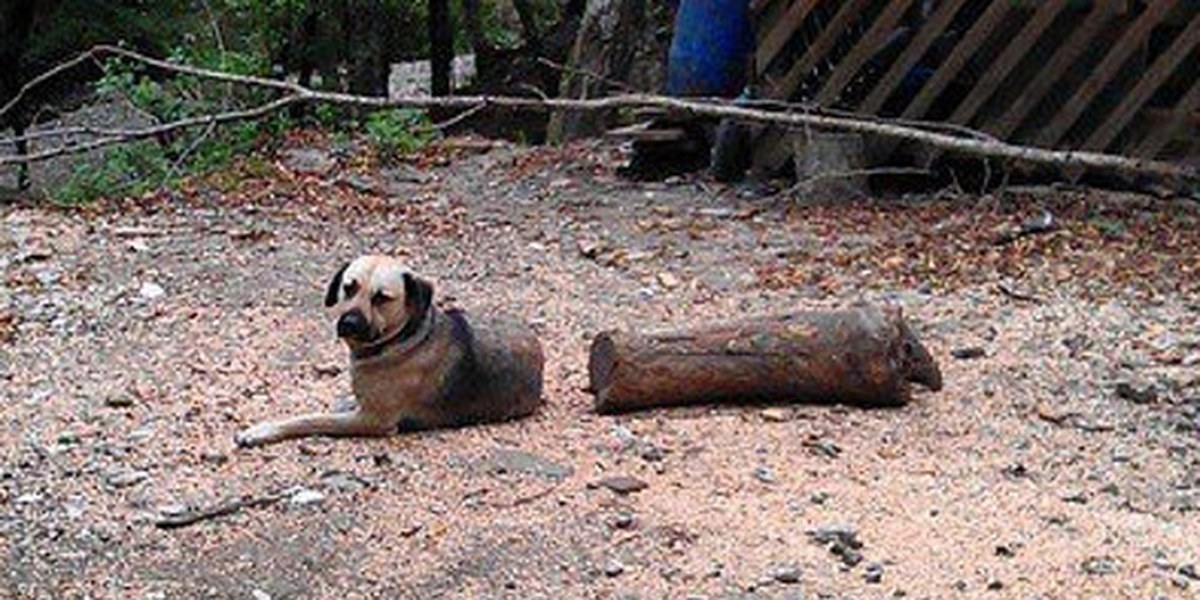
\includegraphics[scale=.13]{Lecture 8 Picture.jpg}
  \end{center}
}



\frame{
  \frametitle{That's it. Thanks for being here. }

  \begin{center}
    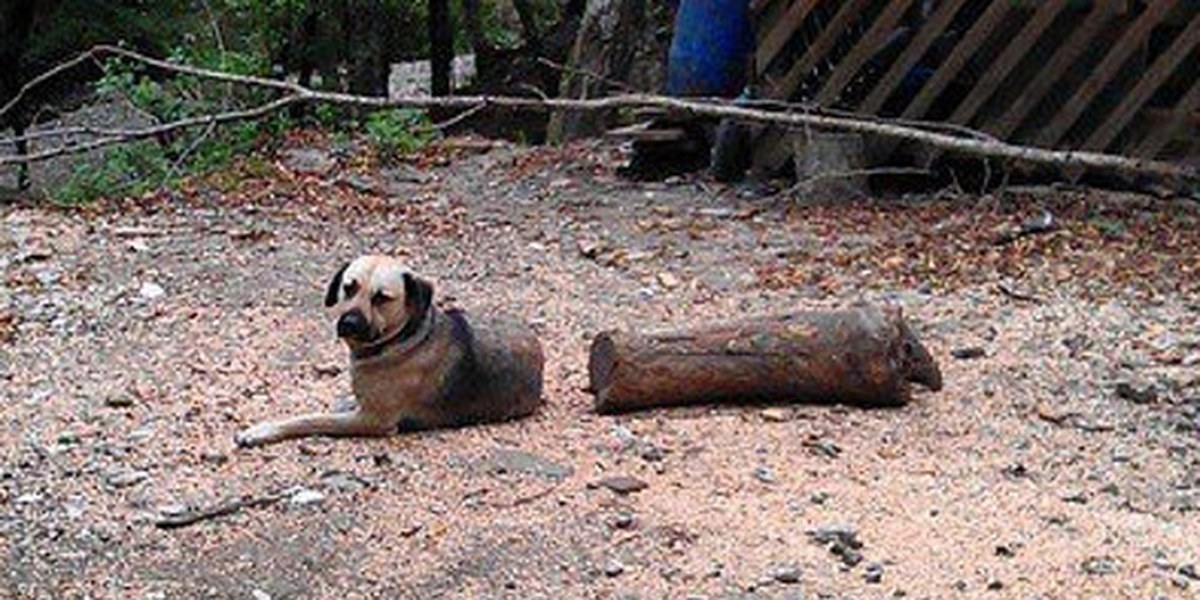
\includegraphics[scale=.25]{Lecture 8 Picture.jpg}
  \end{center}
}




\end{document}


